\subsection{Property View Models}


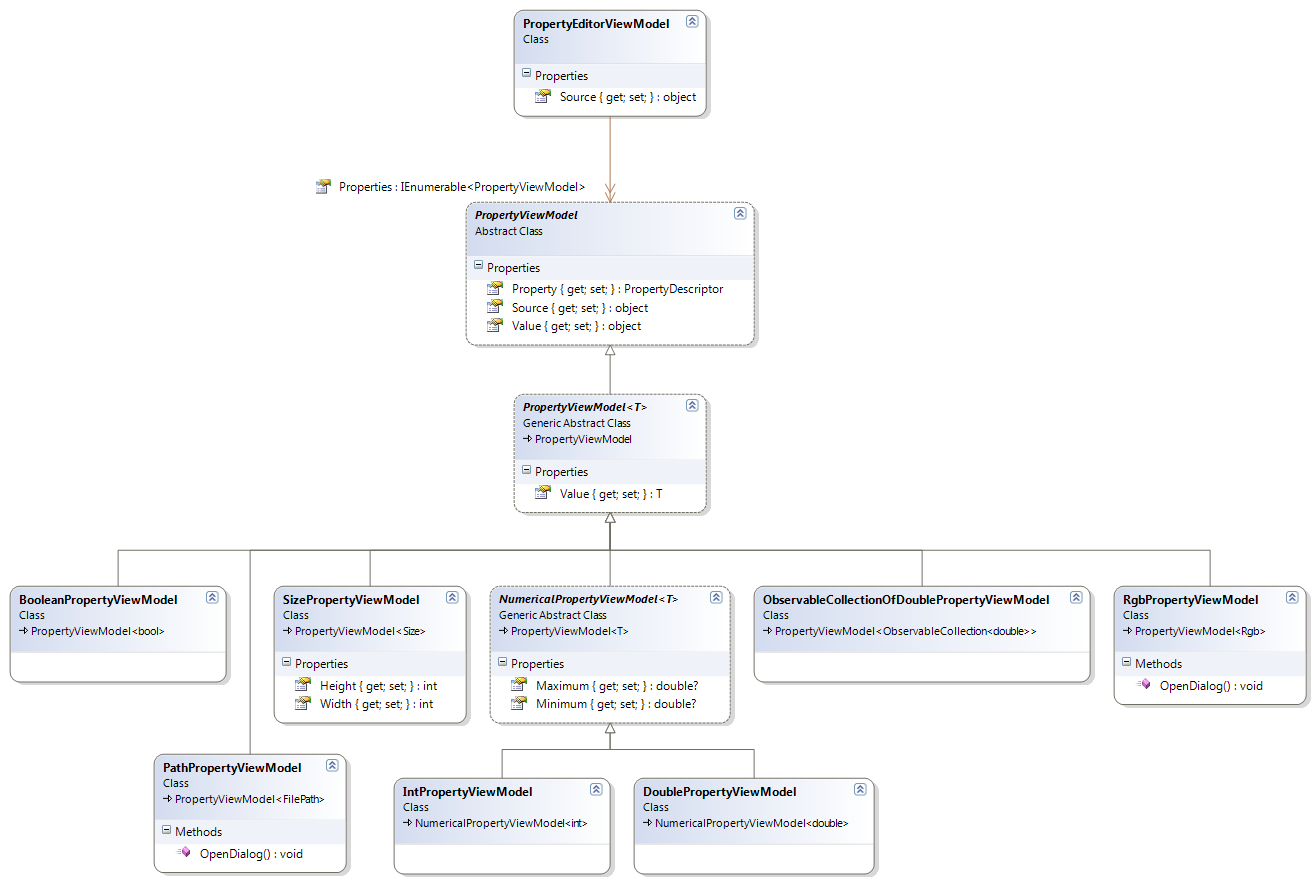
\includegraphics[width=\textwidth]{YuvKA.ViewModel.PropertyEditor/propertyEditor.png}



\subsubsection{YuvKA.ViewModel.PropertyEditor.PropertyViewModel}

\begin{verbatim}
public abstract class PropertyViewModel
\end{verbatim}

\paragraph{Beschreibung}~\\
insert description

\paragraph{Typmember}
\begin{itemize}

\property{Properties}
	\begin{verbatim}
	public IEnumerable<PropertyViewModel> { get; set; }
	\end{verbatim}
	
\property{Property}
	\begin{verbatim}
	public PropertyDescriptor Property { get; set; }
	\end{verbatim}

\property{Source}
	\begin{verbatim}
	public object Source { get; set; }
	\end{verbatim}

\property{Value}
	\begin{verbatim}
	public object Value { get; set; }
	\end{verbatim}

\end{itemize}




\subsubsection{YuvKA.ViewModel.PropertyEditor.PropertyEditorViewModel}

\begin{verbatim}
public class PropertyEditorViewModel
\end{verbatim}

\paragraph{Beschreibung}~\\
insert description

\paragraph{Typmember}
\begin{itemize}

\property{Source}
	\begin{verbatim}
	public object Source { get; set; }
	\end{verbatim}

\end{itemize}




\subsubsection{YuvKA.ViewModel.PropertyEditor.PropertyViewModel<T>}

\begin{verbatim}
public generic abstract class PropertyViewModel<T>
\end{verbatim}

\paragraph{Beschreibung}~\\
insert description

\paragraph{Typmember}
\begin{itemize}

\property{Value}
	\begin{verbatim}
	public T Value { get; set; }
	\end{verbatim}

\end{itemize}




\subsubsection{YuvKA.ViewModel.PropertyEditor.BooleanPropertyViewModel}

\begin{verbatim}
public class BooleanPropertyViewModel
\end{verbatim}

\paragraph{Beschreibung}~\\
insert description



\subsubsection{YuvKA.ViewModel.PropertyEditor.PathPropertyViewModel}

\begin{verbatim}
public class PathPropertyViewModel
\end{verbatim}

\paragraph{Beschreibung}~\\
insert description

\paragraph{Typmember}
\begin{itemize}

\method{OpenDialog}
	\begin{verbatim}
	public void OpenDialog()
	\end{verbatim}

\end{itemize}




\subsubsection{YuvKA.ViewModel.PropertyEditor.SizePropertyViewModel}

\begin{verbatim}
public class SizePropertyViewModel
\end{verbatim}

\paragraph{Beschreibung}~\\
insert description
\paragraph{Typmember}
\begin{itemize}
	
\property{Height}
	\begin{verbatim}
	public int Height { get; set; }
	\end{verbatim}

\property{Width}
	\begin{verbatim}
	public int Width { get; set; }
	\end{verbatim}

\end{itemize}




\subsubsection{YuvKA.ViewModel.PropertyEditor.NumericalPropertyViewModel<T>}

\begin{verbatim}
public generic abstract class NumericalPropertyViewModel<T>
\end{verbatim}

\paragraph{Beschreibung}~\\
insert description

\paragraph{Typmember}
\begin{itemize}

\property{Maximum}
	\begin{verbatim}
	public Nullable<double> Maximum
	\end{verbatim}

\property{Minimum}
	\begin{verbatim}
	public Nullable<double> Minimum
	\end{verbatim}

\end{itemize}




\subsubsection{YuvKA.ViewModel.PropertyEditor.IntPropertyViewModel}

\begin{verbatim}
public class IntPropertyViewModel
\end{verbatim}

\paragraph{Beschreibung}~\\
insert description




\subsubsection{YuvKA.ViewModel.PropertyEditor.DoublePropertyViewModel}

\begin{verbatim}
public class DoublePropertyViewModel
\end{verbatim}

\paragraph{Beschreibung}~\\
insert description




\subsubsection{YuvKA.ViewModel.PropertyEditor.ObservableCollectionOfDoublePropertyViewModel}

\begin{verbatim}
public class ObservableCollectionOfDoublePropertyViewModel
\end{verbatim}

\paragraph{Beschreibung}~\\
insert description



\subsubsection{YuvKA.ViewModel.PropertyEditor.RgbPropertyViewModel}

\begin{verbatim}
public class RgbPropertyViewModel
\end{verbatim}

\paragraph{Beschreibung}~\\
insert description

\paragraph{Typmember}
\begin{itemize}
	
\method{OpenDialog}
	\begin{verbatim}
	public void OpenDialog()
	\end{verbatim}

\end{itemize}


